\chapter{Experiments}

For any execution of an \aspop{} solver, ultimately two distinct metrics of interest exist, \textit{runtime} and \textit{output quality}. While the concept of runtime is intuitive enough, quality is a subjective measure from the perspective of the solver's realistic use cases. It is in the best interest of the end user if the system performs fastest for the tasks it will actually be applied to. 

As the algorithm underlying our \aspop{} solver is exact, the output \gls{solution} set is a predictable function of the parameters it is given; However, this simply moves the optimization of \textit{output quality} to the selection of the program's input parameters. As such, \textbf{phase~1} deals with understanding the mapping from these parameters to output quality.
 
Once the `optimal' user-defined parameters have been established from phase~1, further iteration on the design of the solver can be done to maximize speedup for these expected cases; This effectively fixes the input parameters going forwards. \textbf{Phase~2} seeks to understand the limitations on the speed of the solver as a function of the properties inherent to the input \textit{data set}. The constraints on the parameters provided by phase~1 allow certain implementation decisions involving trade-offs to be made, intended to optimize the speed of the system \textit{specifically} for expected use cases (insofar as the fixed parameters define). Any effects of these alterations to the implementation are followed up with comparative tests.
 
Entering \textbf{phase~3} of the experiments, the \aspop{} solver's implementation is considered final. Ultimately, this last phase conducts comparative experiments between our system and other existing technologies \textsc{blast}~\cite{blast} and Minimap~\cite{minimap} to quantify its comparative performance in terms of runtime and output quality.

Raw experiment data is available at \url{https://github.com/sirkibsirkib/rust_overlaps_data}.

\section{Phase 1: Input Parameter Tuning for Output Quality}
\label{phase1}

\subsection{Goal}
Phase 1 of the experiments seeks to quantify the effects of running the system with different combinations of input parameters. The reasons for this are twofold:

\begin{enumerate}
\item Firstly, it grounds these esoteric parameters \gls{error rate} limit (\bfit{e}) and prefix length threshold (\bfit{t}) in reality, allowing the user to gain an understanding of how to get the most out of the solver.

\item Secondly, it allows the experiments in Phase 2 and Phase 3 the assumption of a constrained possibility space. Assuming users are after high \textit{quality} output solutions with respect to the expected use case, it becomes possible to affix \bfit{t} and \bfit{e}; This allows more targeted testing and optimization such that the system achieves optimal speed specifically for these expected use cases.
\end{enumerate}

\subsection{Experimental Design}
Our definition of \textit{output quality} is based on \textit{F-measure}\footnote{$\text{\textit{F-measure}} = 2 \cdot{} precision \cdot{} recall / (precision + recall)$} which seeks to incorporate precision and recall; Counts for \textit{true positive}, \textit{false positive} etc. are  defined with respect to \glspl{solution} from a predetermined \textit{ground truth} solution set, which is the set of overlaps whose strings really do come from overlapping regions of the \gls{source genome}. To approximate a realistic instance of such true solutions, the data set is constructed from simulated reads from a \textit{real} genome sequence of an HIV-1 reference strain (HXB2), introducing errors according to an \textit{error profile} designed to model the physical nucleotide-reading process. In our case, the ground truth set consists of 4,854,458 unique overlap \glspl{solution}.

High recall is desirable for sequence assembly, as it directly corresponds with how effectively the system utilizes the \glspl{genome copy} of the \gls{source genome} (measured as data set \gls{coverage}). \textit{False negative} solutions reduce recall, and when used for sequence assembly, could potentially prevent the formation of a good overlap chain, and consequentially, result in a less-satisfactory assembly.

High precision is also desirable, as it reduces the run time of any tool that needs to filter out \textit{false positive} solutions. Some use cases might also find false positive overlaps undesirable, as they might negatively impact their own output quality or runtime.


\FloatBarrier

\subsection{Results}
The recall and precision of individual \aspop{} solver executions can be seen in Figure \ref{fig:phase1_plots}, with a 3D surface for recall, and another for precision; Figure \ref{fig:phase1_02} plots the corresponding values for f-measure. Throughout all surfaces, the same $(\bfit{t}, \bfit{e})$ coordinates correspond with the same execution's output set.


\begin{figure}
\centering
   \begin{subfigure}[b]{0.8\textwidth}
   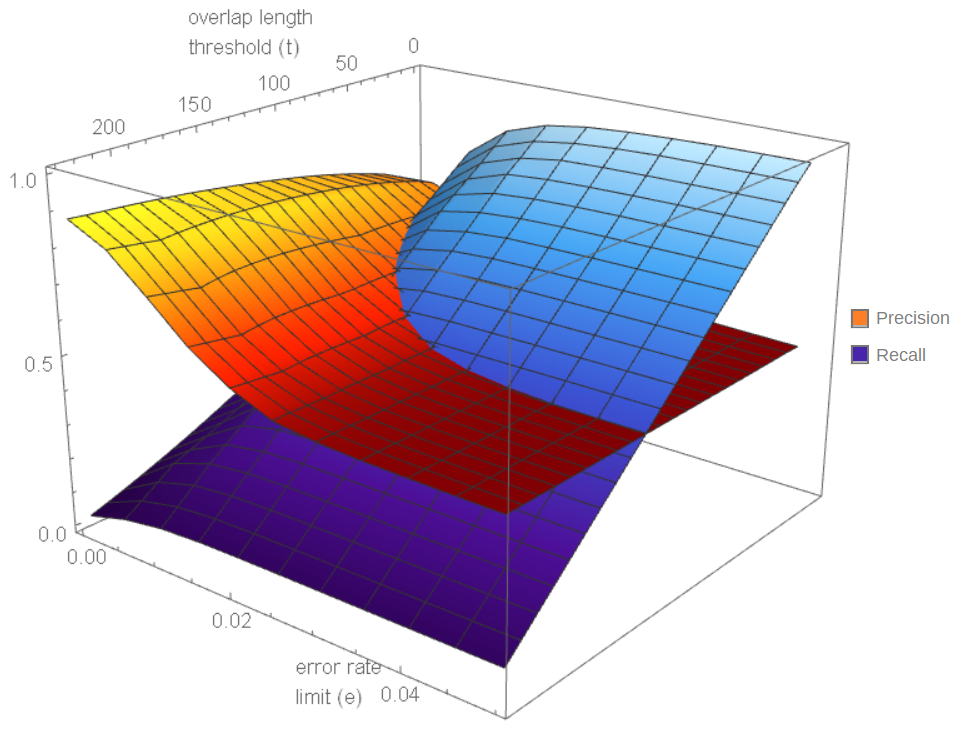
\includegraphics[width=1\linewidth]{images/phase1_A.png}
   \caption{}
\end{subfigure}

\begin{subfigure}[b]{0.8\textwidth}
   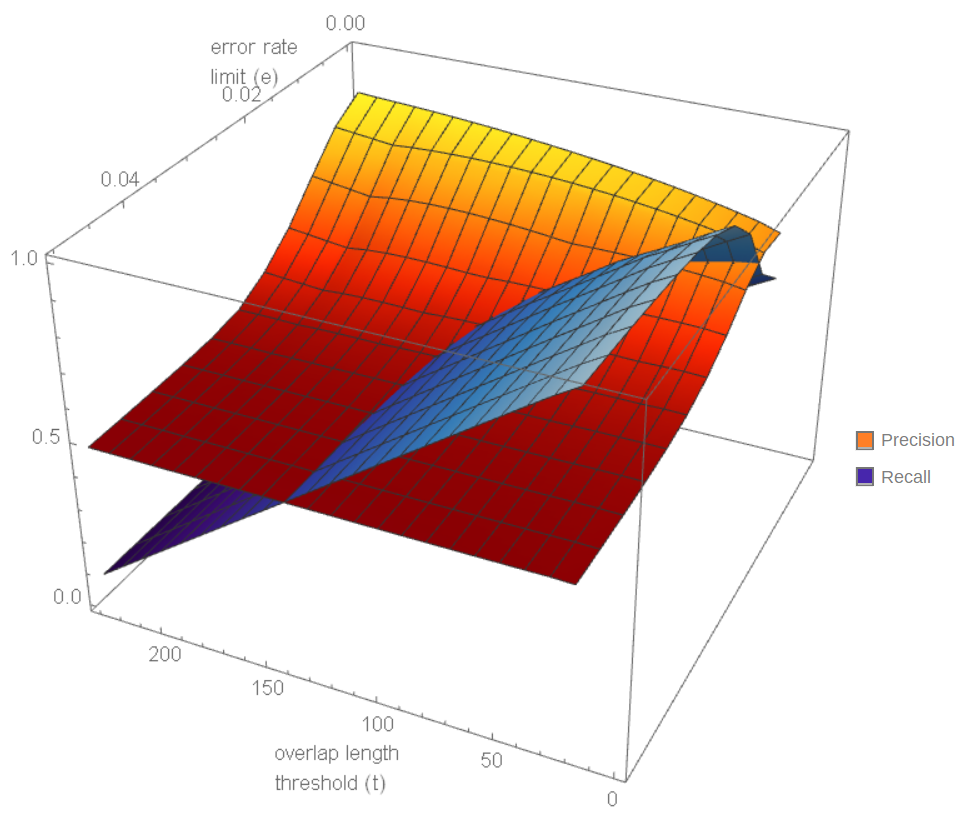
\includegraphics[width=1\linewidth]{images/phase1_B.png}
   \caption{}
\end{subfigure}

\caption[Precision and recall for output solution sets generated from runs using various \bfit{e} and \bfit{t} values.]{(a) Precision and recall for output solution sets generated from runs using various \bfit{e} and \bfit{t} values. (b) Alternative view.}
\label{fig:phase1_plots}
\end{figure}
\subsection{Observations}

As was expected, Figure \ref{fig:phase1_plots} shows that the solver achieves highest recall with restrictions relaxed as much as possible (low \bfit{t} and high \bfit{e}).

Outputs with the highest precision scores were the ones in which only \glspl{solution} \textit{highly} likely to be real were output.
\begin{enumerate}
\item Solutions that have longer overlaps are more likely to be real, explaining the correlation between high \bfit{t} and high precision.
\item Solutions that represent overlaps with very few errors are more likely to be real. Increased error blurs the distinction between different subsequences of the genome, increasing the number of false positives.
\end{enumerate}

Beyond approximately 3\% error, not much seems to change with respect to either metric, as can be seen in the `plateauing' of both recall and precision surfaces.

Clearly there is a trade-off between recall and precision to be considered when selecting one's input parameters. As very low values for either are highly undesirable, the values for run \textit{F-measures} in figure \ref{fig:phase1_02} give a view of the relative \textit{quality} of each run, factoring in the contributions of both recall and precision.


\begin{figure}[!htb]
\centering
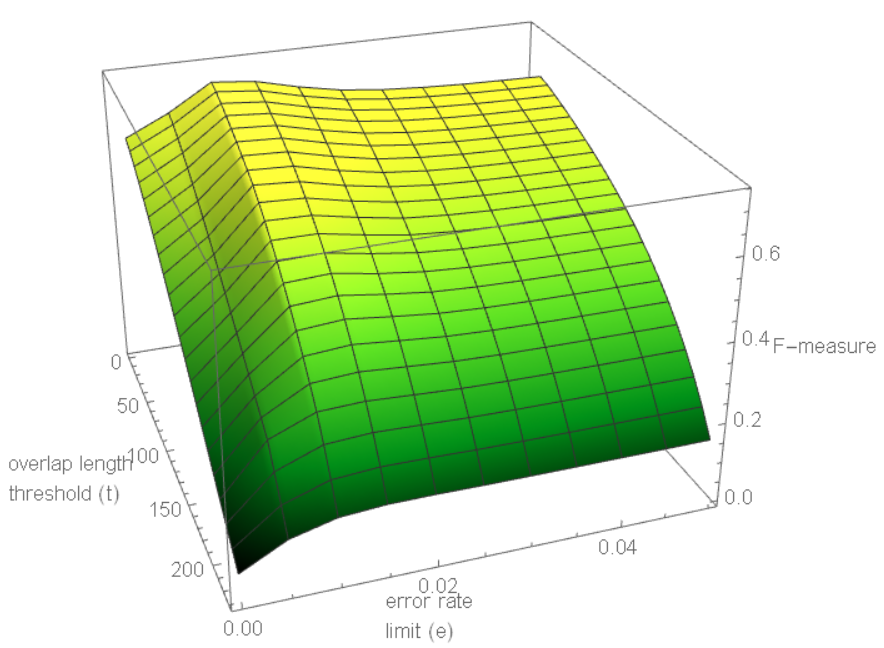
\includegraphics[width=0.9\textwidth]{images/fmeasure.png}
\caption{F-measure of output solution sets generated from runs using various \bfit{e} (error rate limit) and \bfit{t} (overlap threshold length) values.}
\label{fig:phase1_02}
\end{figure}

Use of shorter \bfit{t} appears to be consistently beneficial, and the choice of \bfit{e} seems optimal at approximately 1.2\% regardless of \bfit{t}. As exceptionally short overlap threshold of $< 80$ is undesirable for sequence assembly of viral genomes\footnote{See Section \ref{context} for more information on this choice of threshold.} (our primary use case), the optimal choice of parameters seems to be:
\begin{align*}
\bfit{t} &= 80\\
\bfit{e} &= 1.2\%
\end{align*}

\FloatBarrier

\section{Phase 2: Runtime Optimization Under Expected Conditions}
\label{phase2}

\subsection{Goal}
Experiments in this phase seek to tease out relationships between properties of the input data and runtime. Runtime on its own is a rather coarse measurement. For our \aspop{} solver, there are two logical means of fragmenting runtime into its principal components:

\begin{enumerate}
\item per \gls{suffix filter} block length

Patterns perform several \glspl{query} to the \gls{text index}, each with a different length of \gls{filter}. Aggregating like-sized filters will allow us a view into how filters of different lengths share the load of solving the problem, and identify algorithmic bottlenecks related to filters of only certain lengths.

\item per \gls{filter algorithm} step

The \gls{search step}'s runtime is a function of the shape of the query-search trees for each \gls{pattern}, which is in turn a function just about everything. The verification time is dependent on the number of \glspl{candidate} from the search step, as well as the rate at which candidates are \textit{spurious}.
\end{enumerate}

Very many properties can be extracted from a data set and reasoned over. Identifying the implications of properties that are \textit{intuitive} provides insight into what is actually happening inside the solver. Four such properties were identified and tested:

\begin{enumerate}
\item Genome Length

The length of the \gls{source genome} mostly affects the number of \glspl{read} in the data set without greatly\footnote{The impact of genome length on runtime is small when compared to a comparable increase in coverage, the most similar data set property. This is because both properties increase the number of reads to the same degree, but coverage usually introduces highly \textit{similar} reads leading to more text index hits and more overlap solutions.} impacting the number of overlaps per read. More reads also mean a longer \gls{text}, which has the side effect of more text index `hits', reducing pruning in query search trees. Unless otherwise specified, genome length is kept consistently at around 9600 nucleotides.

\item Read Length

Read length controls the \textit{maximum} length of a read (some fragments end up shorter). Read length is determined \textit{independently} to source genome length and \gls{coverage}; As the read length increases, the number of reads in the data set decreases. This is truly a measure of the \textit{fragmentation} of the source genome, not to be confused with coverage. Except in this experiment where it is the response variable, read length is consistently kept at approximately 250bp  (base pairs).

\item Coverage

Coverage is a measure of the number of \glspl{genome copy} composing the data set\footnote{Coverage has different specific definitions depending on the source. See the glossary definition of `coverage' for details. For our purpose, it is sufficient to consider coverage to be uniform across the length of the genome, being analogous to the count of genome copies in the data set.}. With a higher-coverage data set, there are more reads and more overlaps (in the \gls{search step} as well as the resulting \gls{solution} set). When not otherwise specified, experimental data sets have 500x coverage.

\item Divergence

If reads in a dataset are drawn from more than one source genome, one can reason about these genomes' divergence with respect to one another. Genomes with low divergence have a lot in common, and will contain more of the same substrings; A data set built from low-divergence genomes will likely result in more overlaps being found. For the coverage and divergence experiments, the data is drawn from real sources, with unknown constant values of coverage. For the other two experiments divergence is not defined, as only one source genome was used.

\end{enumerate}

\subsection{Experimental Design}
A battery of four experiment \textit{groups} tested the same target variables, but each time in response to a different \textit{data set property}. For each group, two experiments were performed:

\begin{enumerate}
\item Total runtimes (along with runtimes fragmented per \gls{filter algorithm} step) shown according to the given predictor variable.

\item Proportion of total runtime distributed across different \gls{filter} lengths, plotted across values of the predictor variable.
\end{enumerate}

% \FloatBarrier
\subsection{Results}
Figures \ref{fig:gnmlen} - \ref{fig:div} show the effect the various properties of the data set had on the runtime, as seen in two different partitions: per \gls{filter algorithm} step and per \gls{filter} blocks.



\begin{figure}
\centering
\makebox[\linewidth][c]{%
\begin{subfigure}[t]{.53\textwidth}
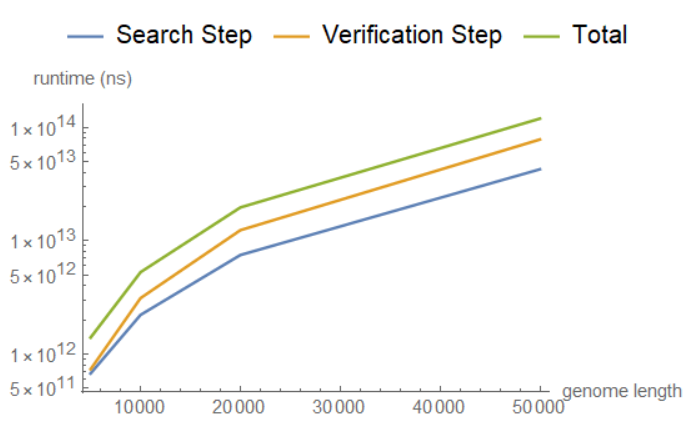
\includegraphics[width=1\linewidth]{images/gnmlen_a.png}
\caption{}
\end{subfigure}
~
\begin{subfigure}[t]{.53\textwidth}
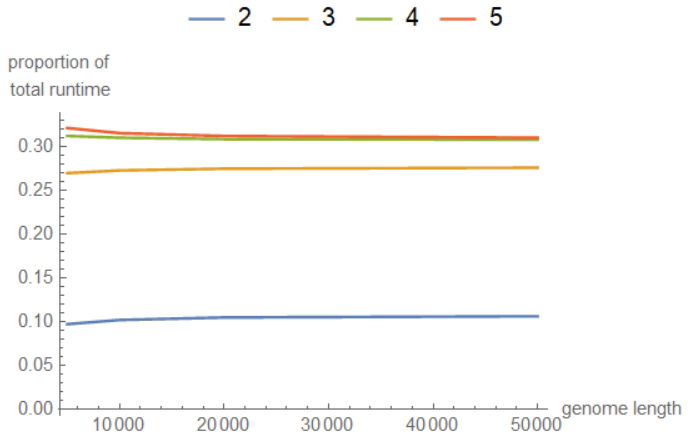
\includegraphics[width=1\linewidth]{images/gnmlen_b.png}
\caption{}
\end{subfigure}
}
\caption[Work time of \aspop{} solver runs partitioned into principal components, plotted as a function of \textit{genome length}]{Work of \aspop{} solver runs partitioned into principal components, plotted as a function of \textit{genome length}.\\(a) Total runtime (in nanoseconds) partitioned by filter algorithm step.\\(b) Runtime proportion partitioned by suffix filter block lengths.}
\label{fig:gnmlen}
\end{figure}



\begin{figure}
\centering
\makebox[\linewidth][c]{%
\begin{subfigure}[t]{.53\textwidth}
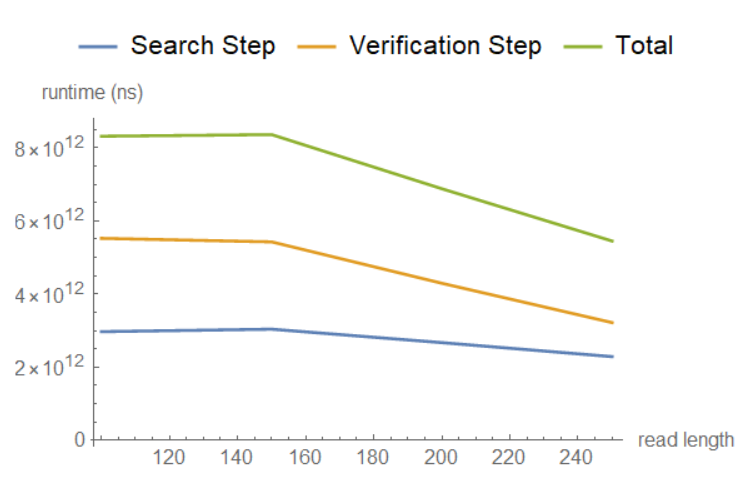
\includegraphics[width=1\linewidth]{images/rdlen_a.png}
\caption{}
\end{subfigure}
~
\begin{subfigure}[t]{.53\textwidth}
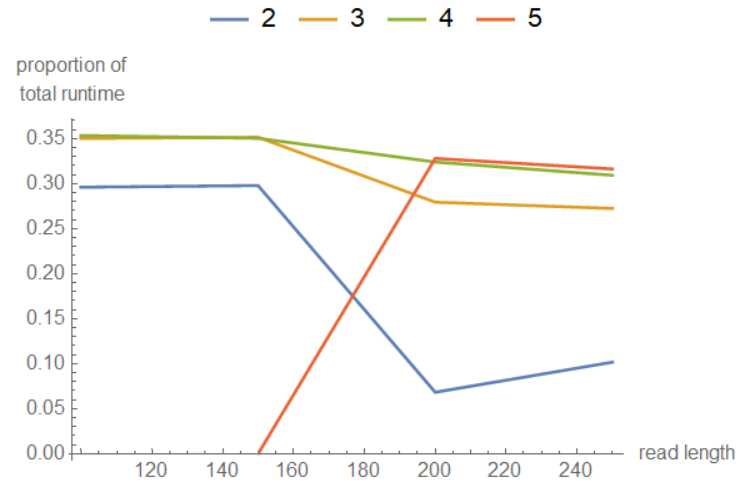
\includegraphics[width=1\linewidth]{images/rdlen_b.png}
\caption{}
\end{subfigure}
}
\caption[Work time of \aspop{} solver runs partitioned into principal components, plotted as a function of \textit{read length}]{Work of \aspop{} solver runs partitioned into principal components, plotted as a function of \textit{read length}.\\(a) Total runtime (in nanoseconds) partitioned by filter algorithm step.\\(b) Runtime proportion partitioned by suffix filter block lengths.}
\label{fig:rdlen}
\end{figure}



\begin{figure}
\centering
\makebox[\linewidth][c]{%
\begin{subfigure}[t]{.53\textwidth}
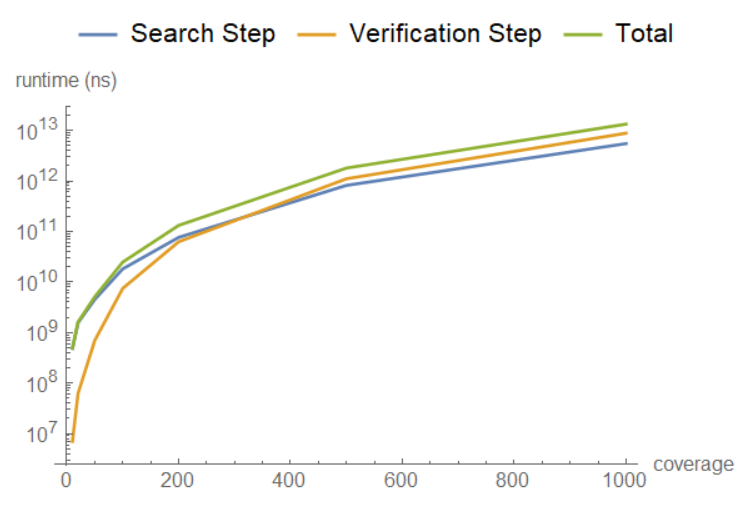
\includegraphics[width=1\linewidth]{images/cov_a.png}
\caption{}
\end{subfigure}
~
\begin{subfigure}[t]{.53\textwidth}
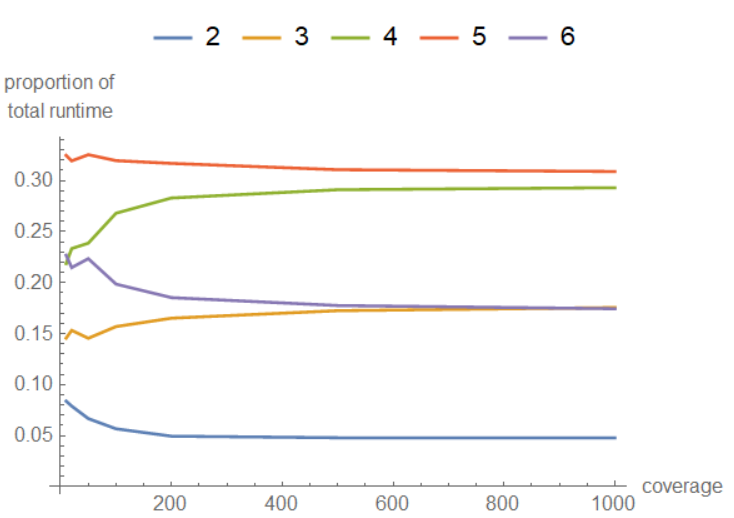
\includegraphics[width=1\linewidth]{images/cov_b.png}
\caption{}
\end{subfigure}
}
\caption[Work time of \aspop{} solver runs partitioned into principal components, plotted as a function of \textit{genome coverage}]{Work of \aspop{} solver runs partitioned into principal components, plotted as a function of \textit{genome coverage}.\\(a) Total runtime (in nanoseconds) partitioned by filter algorithm step.\\(b) Runtime proportion partitioned by suffix filter block lengths.}
\label{fig:cov}
\end{figure}



\begin{figure}
\centering
\makebox[\linewidth][c]{%
\begin{subfigure}[t]{.53\textwidth}
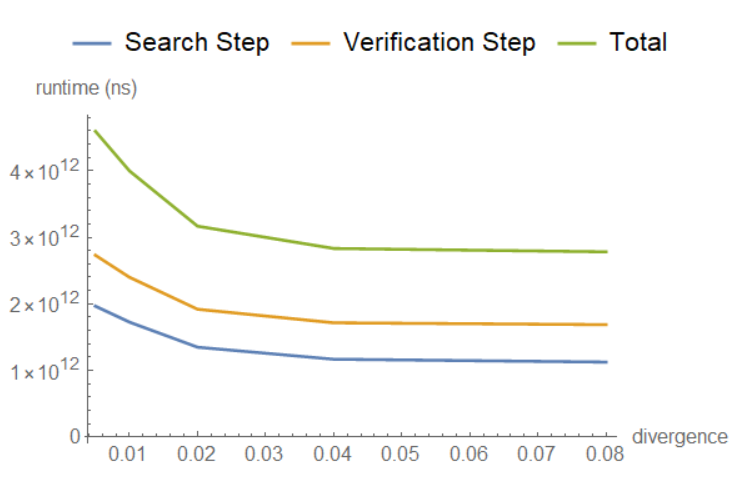
\includegraphics[width=1\linewidth]{images/div_a.png}
\caption{}
\end{subfigure}
~
\begin{subfigure}[t]{.53\textwidth}
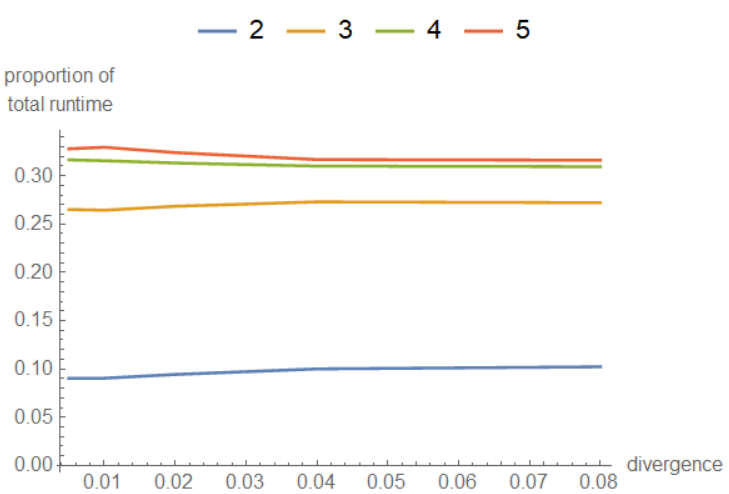
\includegraphics[width=1\linewidth]{images/div_b.png}
\caption{}
\end{subfigure}
}
\caption[Work time of \aspop{} solver runs partitioned into principal components, plotted as a function of \textit{genome divergence}]{Work of \aspop{} solver runs partitioned into principal components, plotted as a function of \textit{genome divergence}.\\(a) Total runtime (in nanoseconds) partitioned by filter algorithm step.\\(b) Runtime proportion partitioned by suffix filter block lengths.}
\label{fig:div}
\end{figure}

\FloatBarrier

\subsection{Observations}

Increased \textit{read length} in fig \ref{fig:rdlen} (a) demonstrated that for the same amount of data overall, the algorithm \textit{sped up} when faced with a smaller number of longer \glspl{read}, but not to an extreme extent. From (b), one can observe the longer \glspl{filter} beginning to `kick in' only for longer read lengths, as would be expected. It is notable here that filters took time roughly correspondent to their length. This is desirable behavior as it indicates that the workload is evenly distributed amongst filters (as much as their varying lengths will allow) and that no obvious niche cases are causing overwhelming slowdown. 
\begin{figure}[]
\centering
\makebox[\linewidth][c]{%
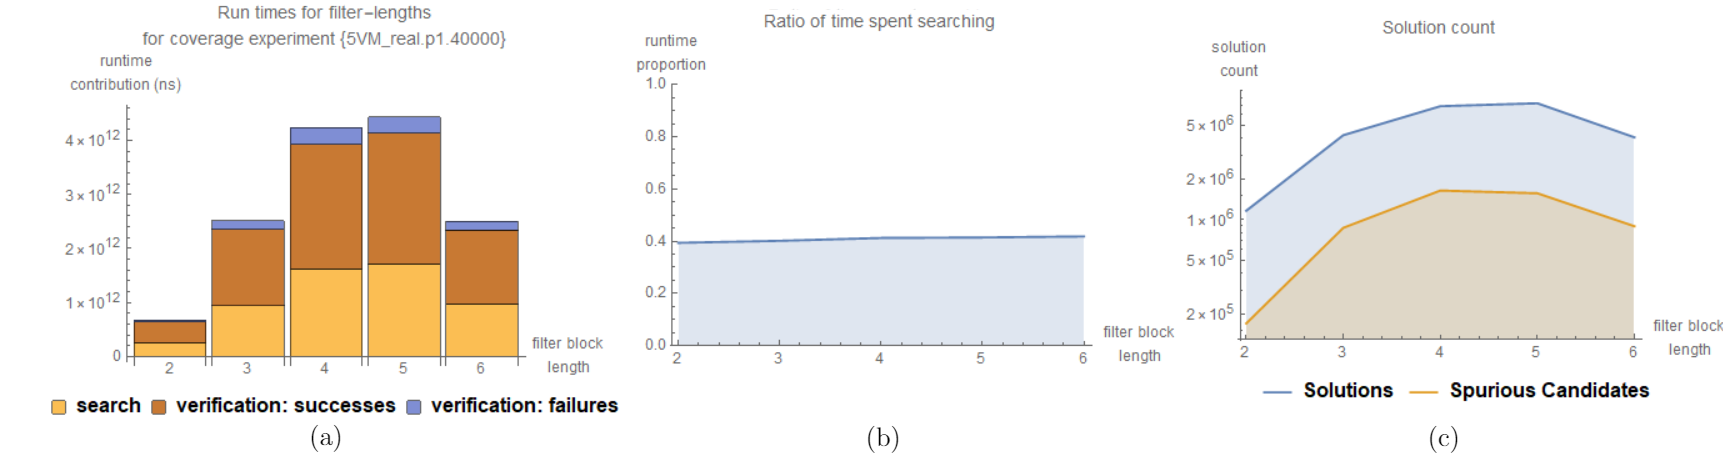
\includegraphics[width=1.3\textwidth]{images/cov40k_details.png}
}
\caption[Details of runtime for run `dataset\_coverage\_1000x'.]{Details of runtime for run `dataset\_coverage\_1000x'.\\(a) Runtime contributions for steps of the filter algorithm.\\(b) Ratio of time spent searching per filter block length.\\(c) Solution counts that did and did not verify per filter block length.}
\label{fig:cov40k_details}
\end{figure}
Increased \gls{coverage} proportionately increases the size of a data set, but increases the size of the \gls{solution} set super-linearly. As such, it is interesting to observe in Figure \ref{fig:cov} (a) that both steps of the \gls{filter algorithm} do not increase in lockstep, but the \gls{verification step} overtakes the \gls{search step} in runtime for high-coverage data. This was also visible in Figure \ref{fig:gnmlen} (a). Figure \ref{fig:cov} (b) Shows a trend for medium-length filters to contribute more to run time; Figure \ref{fig:cov40k_details} observes this in more detail, and shows that it is justified, with filters consistently spending more time working when they find more \glspl{solution}. Longest filters are shown to find fewer solutions than medium-length filters; This could be due to patterns differing in lengths and, consequently, several patterns simply not having a 6th filter to contribute to the overall runtime and solution set. The stabilizing proportions in Figure \ref{fig:cov} (b) are best explained as the law of large numbers at work; With low coverage (a smaller read set), the work contribution proportions are rather unstable. Why exactly these proportions seem to gravitate to fixed positions in a continuous direction and not in a zig-zagging fashion is unknown.




Increased \textit{divergence} in Figure \ref{fig:div} (a) was marked with a consistent reduction in overall runtime. This is to be expected as the data set's \glspl{source genome} have fewer overlaps in common, causing a more spindly search tree in the \gls{search step} as \glspl{match location} dry up. The  behavior of the individual filters remained relatively consistent for filters across the values of divergence. Figure \ref{fig:div} (b) shows that the distribution of work remains remarkably stable, maintaining the predicted relative positions across different solver executions.

\FloatBarrier
\section{Phase 3: Comparison to Other Solvers}
\label{phase3}

\subsection{Goal}
At the end of Phase 2 in Section \ref{phase2}, the implementation for our \aspop{} solver was considered final; This last phase tests how it compares to some existing solvers (namely \textsc{blast} and Minimap) in terms of \textit{output quality}\footnote{As with Phase 1 in Section \ref{phase1}, quality is defined in terms of \textit{F-measure} $=  2\cdot{}precision\cdot{}recall/(precision+recall)$.} and runtime in much the same way as in phase~1.

\textbf{Test 1} represents our primary focus on the use case of an \aspop{} solver in the context of viral genome assembly. Here, desirable \glspl{solution} only come from overlapping regions in the \glspl{source genome}; Only through the discovery of these `true' overlaps can the resulting assembly graph reconstruct these source genomes correctly. As such, the data set selected to represent this use case contains a mix of 5 viral strains. Overlaps found \textit{between} strains are not considered `true', instead counting as false positives and contributing to a diminished measure of precision.

\textbf{Test 2} compares the performance of our \aspop{} solver when applied to human DNA; The intention of this test is to check how runtime and output quality change when the solver is applied to a new type of data set with different properties.

\subsection{Experimental Design}

For each of the two tests, our \aspop{} solver, \textsc{blast} and Minimap were run on the data set sequentially. Many variations of this experiment are conceivable under these conditions, but for our purposes it was most interesting to test the performance of our system in conditions that were found in phase~1 to be conducive to finding the highest-quality solutions set for the purpose of viral genome assembly. As such, runs were done with error rate limit (\bfit{e}) $=$ 1.2\% and threshold overlap length (\bfit{t}) $=$ 80.

All solvers were run on a cluster computer of 24~Intel\textsuperscript{\textregistered} Xeon\textsuperscript{\textregistered} E52620-0s running at~2.00~GHz with 252~GB of storage. Each process was given 10~threads and sufficient free logical cores to run under negligible CPU contention.

The 5-mix of viral genomic data is taken from HXB2 (accession number K03455), available at the NCBI Reference database~\cite{ncbi}. It consists of a sample of 80,000 reads (approximately 2000x coverage) with most reads being of length 250bp.

The human DNA data is taken from Nisk.org's \textit{genome in a bottle} (Individual NA12878)~\cite{genomeinabottle}. Paired-end reads are 2x15 base-pairs at~30x coverage, but with \gls{read} ends truncated of extremely low confidence symbols (resulting in most reads being of length circa 150bp). These reads are taken from a 40,000bp-long subsequence of the MHC region, chromosome~6, base pairs 32,400,000~-~32,800,000.

\subsection{Results}\subsubsection{Viral Genome Data}
\label{p3_viral}

Figure \ref{fig:viral_timespace} shows the properties of the runs for all three solvers, such as the runtime\footnote{Note that runtime is measured \textit{cumulatively} for all running threads in all cores, while wall time is not. This means a well-parallelized program will have a long runtime, but short wall time.} (in terms of user time $+$ system time\footnote{`User time' refers to CPU time spent in user-mode code (outside the kernel) within the process. `System time' refers to CPU time spent in the kernel within the process.}), as well as the total elapsed `wall time' (real-world duration between start and finish of the execution). The peak space\footnote{Similar to runtime, memory usage can also be inflated with response to increased parallelism, as memory of all cores is counted together.} in memory used is also shown.

The Venn diagram given in Figure \ref{fig:viral_venn} shows the \textit{universe} of all unique overlap \glspl{solution} found between all three solvers; Solutions within the \textit{ground truth} set are also shown. Intuitively, a perfect solver's solution set would be equivalent to the ground truth set; Each excluded true solution decreases recall, and each included false solution decreases precision. 

Figure \ref{fig:prec_rec_f_p3} shows the values of recall, precision and \textit{f-measure} for all three solution sets with respect to the ground truth set.

\begin{figure}
\centering
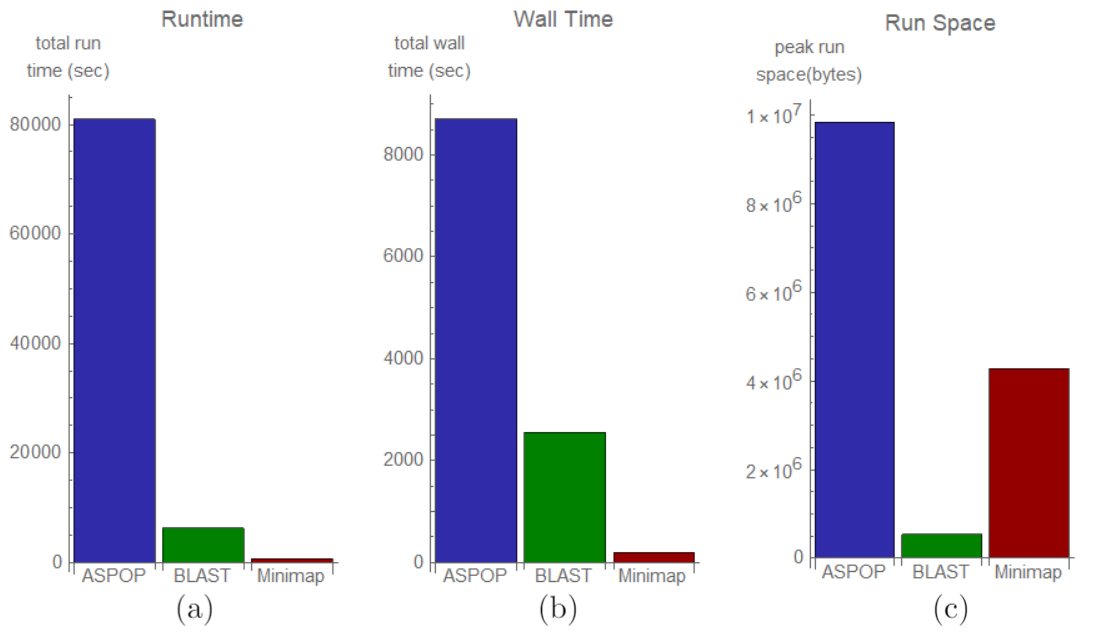
\includegraphics[width=0.85\linewidth]{images/time_space_v.png}
\caption[Time and space usages for runs of three \aspop{} solvers on a moderate data set containing a 5-strain mix of viral strains.]{Time and space usages for runs of three \aspop{} solvers on a moderate data set containing a 5-strain mix of viral strains.\\(a) Runtime of the solver in terms of system and user time in seconds\footnotemark{}.\\(b) Elapsed time as perceived externally in seconds.\\(c) Peak space required during solve in kb.}
\label{fig:viral_timespace}
\end{figure}

\FloatBarrier
\footnotetext{In the previous sections we have used nanosecond-granularity for time measurements, as they were made by a custom \aspop{} benchmarker able to measure time taken by components separately. For this test, we rely on linux's \url{/usr/bin/time} output, which uses second-granularity.}


\begin{figure}
\centering
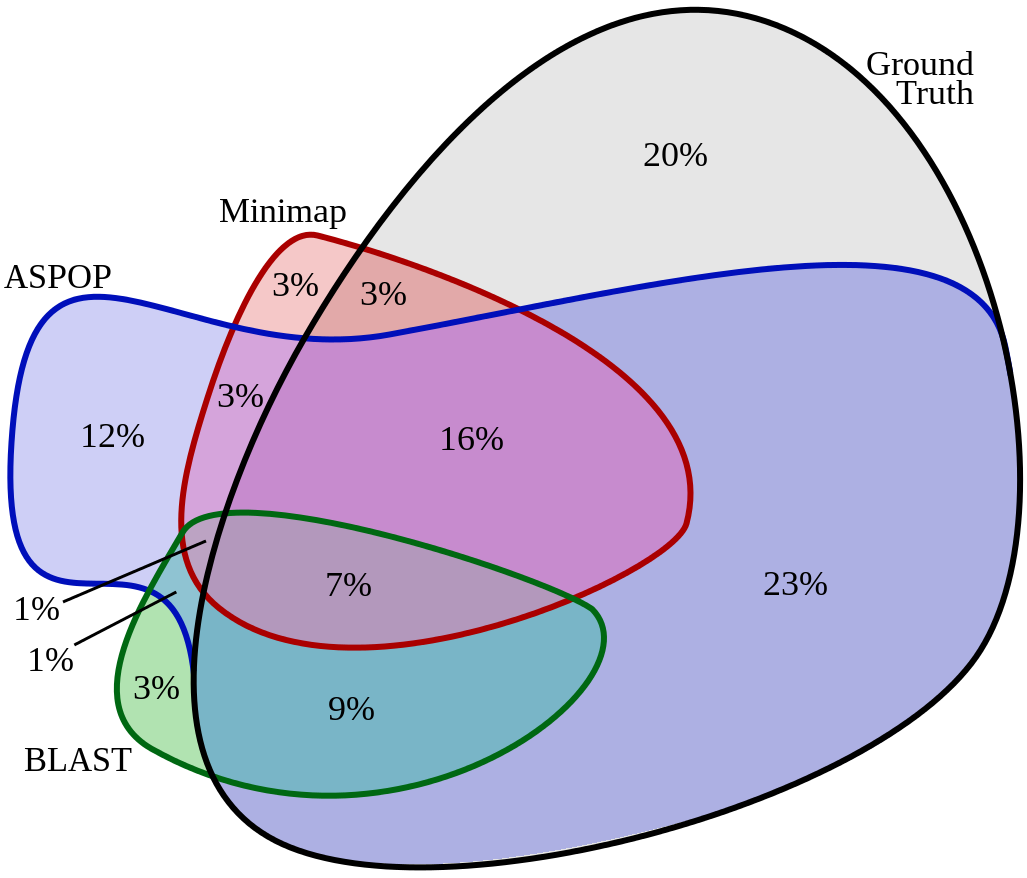
\includegraphics[width=0.55\linewidth]{images/viral_venn.png}
\caption[Venn diagram of solutions common between our \aspop{}, \textsc{blast} and Minimap against the \textit{ground truth} set for for a 5-strain viral mix data set]{Venn diagram of solutions found from a moderate 5-strain viral genome mix using our \aspop{} solver (blue), \textsc{blast} (green), Minimap (red) and the \textit{Ground Truth} (gray). Regions are labeled with the percentage of total solutions found, and are not necessarily to exact scale. Regions whose values round to $< 1\%$ of solutions are not labeled.}
\label{fig:viral_venn}
\end{figure}

\begin{figure}
\centering
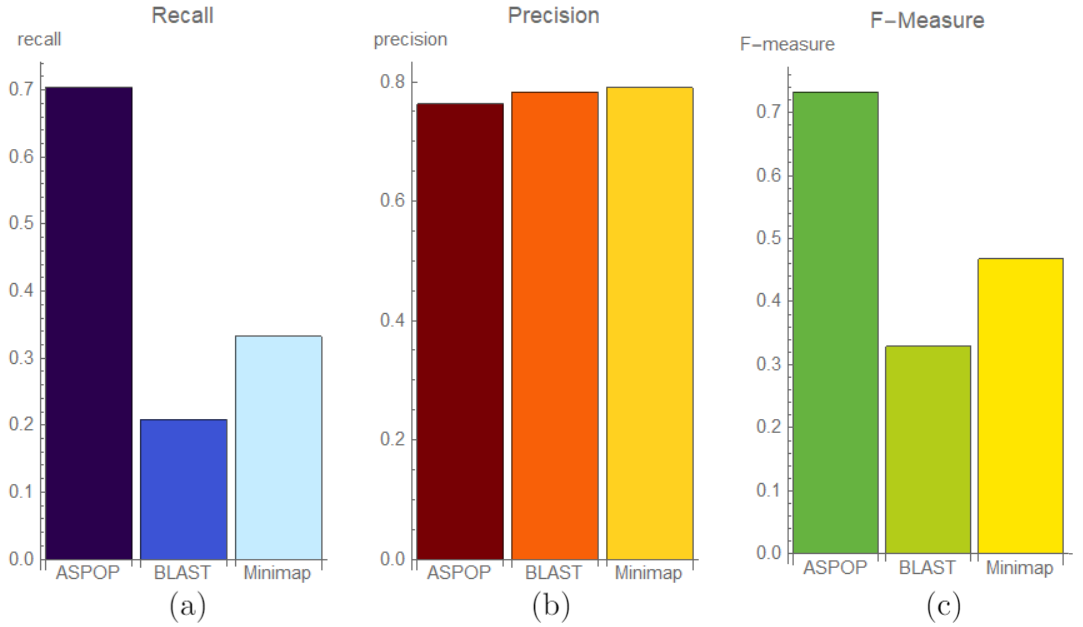
\includegraphics[width=0.9\linewidth]{images/prec_rec_f_p3.png}
\caption[Recall, precision, and f-measure for our \aspop{} solver, \textsc{blast} and Minimap running on a moderate 5-strain mix of viral data.]{Plots of (a) Recall (b) Precision and (c) F-measure for our \aspop{} solver, \textsc{blast} and Minimap running on a moderate 5-strain mix of viral data.}
\label{fig:prec_rec_f_p3}
\end{figure}


% \FloatBarrier


\subsubsection{Human Genome Data}
As in Section \ref{p3_viral} above, Figure \ref{fig:human_timespace} plots values\footnote{As in the previous section, the values of runtime and peak space are sensitive to parallelism. These solvers are parallelized to different degrees so it is important to interpret these measures in the context of wall time to gain a sense of the parallelism influencing the other values.} of runtime, wall time and peak space usage; In this experiment, the solvers were set on a data set containing \glspl{read} from human DNA.

Figure \ref{fig:human_venn} presents a Venn diagram of the \textit{universe} of \glspl{solution} found by all three solvers. Note that unlike the viral experiment, this data set has no known \textit{ground truth} set, as this is not simulated data under our control. As such, this diagram can only hint at the relationships between these solution sets, such as in which ways they are similar, different or how the size\footnote{\textsc{blast}, for instance, can output the same solution numerous times. Only \textit{unique} solutions are considered for these experiments.} between solution sets compare.



\begin{figure}
\centering
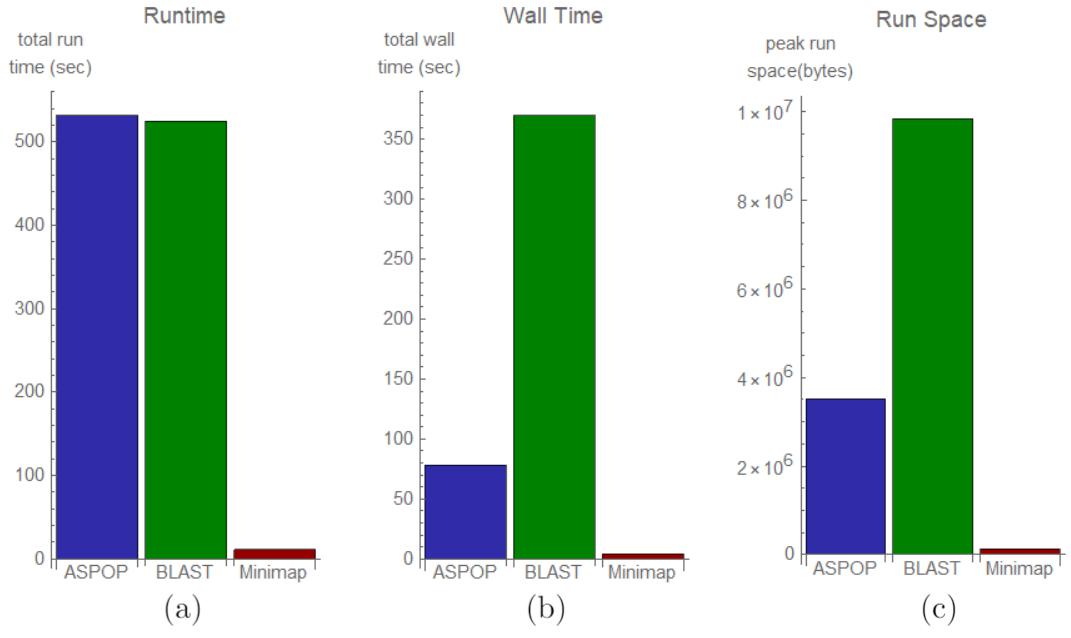
\includegraphics[width=0.9\linewidth]{images/time_space_h.png}
\caption[Time and space usages for runs of three \aspop{} solvers on a moderate data set containing a sample of human DNA]{Time and space usages for runs of three \aspop{} solvers on a moderate data set containing a sample of human DNA.\\(a) Runtime of the solver in terms of system and user time in seconds.\\(b) Elapsed time as perceived externally in seconds.\\(c) Peak space required during solve in kb.}
\label{fig:human_timespace}
\end{figure}

\begin{figure}
\centering
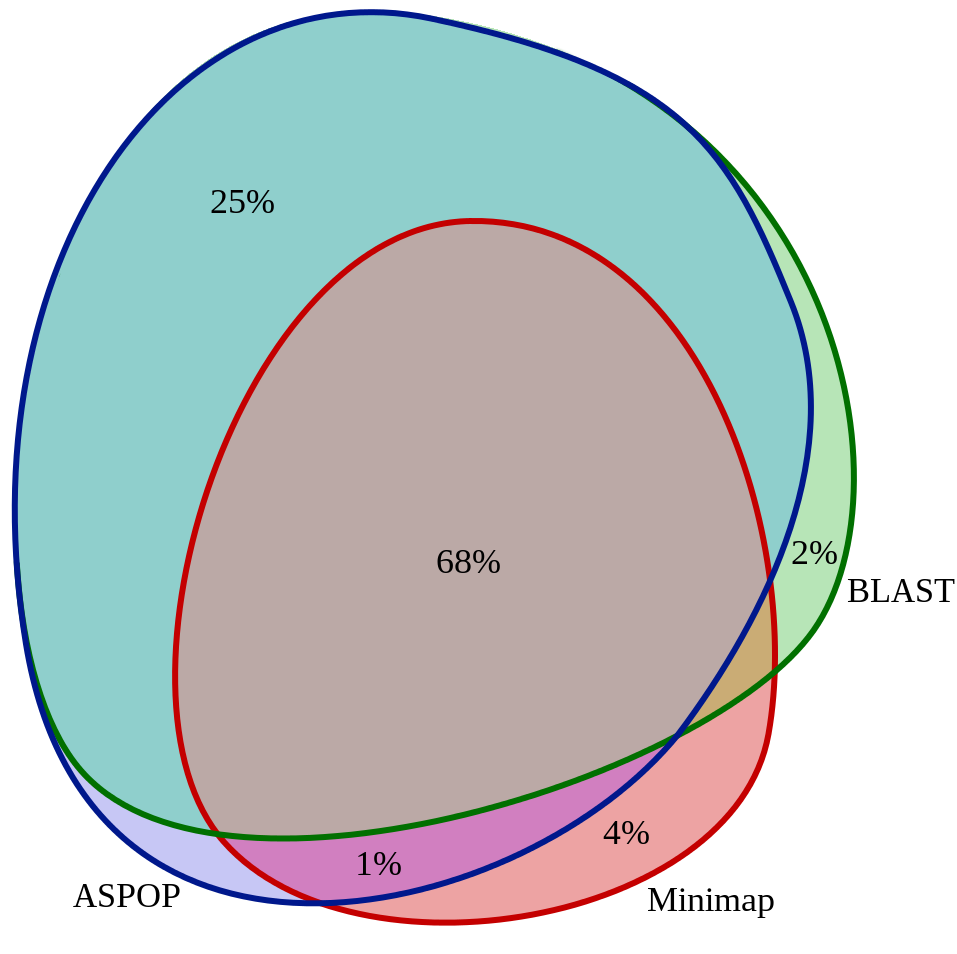
\includegraphics[width=0.5\linewidth]{images/human_venn.png}
\caption[Venn diagram of solutions common between our \aspop{}, \textsc{blast} and Minimap for for a data set of human DNA]{Venn diagram of solutions found from a small data set of human DNA using our \aspop{} solver (blue), \textsc{blast} (green) and Minimap (red). Regions are labeled with the percentage of total solutions found, and are not necessarily to exact scale. Regions whose values round to $< 1\%$ of solutions are not labeled.}
\label{fig:human_venn}
\end{figure}





\subsection{Observations}

Much can be ascertained about our \aspop{} solver, as well as its competitors, from the results of just these two experiments. It is immediately striking that Minimap is \textit{blazingly-fast} despite the fact that it didn't effectively make use of all 10 worker threads. Section \ref{fullmhc} shows that in a larger data set, Minimap's speed superiority becomes even more pronounced. In both cases, Minimap wrote \glspl{solution} in somewhere around 2\% of the time taken for our \aspop{} solver. However, overall, Minimap missed the largest percentage of solutions of all three solvers.

\textsc{blast} seemed to struggle with the human data, experiencing a spike in the wall time as well as peak run space. As this was not the case with the viral data, it seems likely that this is a result of blast struggling with the \textit{genome length}; This is a property with a large value for the human data set \textit{relative} to properties of the viral data set. \textsc{blast} consistently made the poorest use of parallelism, using an average of 230\% of CPU time even with 10 threads and an abundance of cores.

Our \aspop{} solver was generally the slowest solver of the three, specifically for the heftier viral data set. Our \aspop{} solver also had the largest space peak usage. However,  this is likely attributed to its thorough use of the available worker threads in tandem; With space requirements scaled to effective CPU usage, our solver had a smaller peak space usage than \textsc{blast} (and also Minimap in the human data experiment). On the other hand, our solver had the superior \textit{output quality}, represented by the F-measure for the viral experiment, where the \textit{ground truth} set was known. Although solvers were largely indistinguishable in terms of precision, the \aspop{} solver had the highest recall by far. This is almost certainly a direct result of the \gls{suffix filter} algorithm being \textit{exact}, instead of based on heuristics as with the other solvers.

For the \aspop{}, the choice of \bfit{e}$=1.2\%$ was optimal for the purpose of viral genome assembly. This might not necessarily be the case for the other solvers, lending credence to the notion that a user could achieve similar output quality to our solver using, for instance, Minimap but running it with more \textit{lenient} parameters (higher \bfit{e} or lower \bfit{t}); Minimap certainly has the time to spare for finding extra solutions. More work is needed to see if this holds. From what we know so far, it can however be presumed that running any solver with relaxed parameters results in decreased precision. For this reason, beating our solver's F-measure requires not only increased recall, but increased recall \textit{outweighing} the expected decreased precision.









\subsubsection{A Note about Runtime and Peak Run Space}
\label{note:runtime_runspace}

It is immediately apparent that the \aspop{} solver is the slowest; To make matters worse, for this experiment the \textsc{blast} solver had no choice but to find overlaps below the \textit{overlap length threshold} \bfit{t}, (As this is not an exposed parameter for \textsc{blast}) and to discard\footnote{In this decision there was a degree of compromise. If we kept the below-threshold overlaps we risked producing a \textsc{blast} solution set utterly incomparable to our \aspop{} solver's solution set. Alternatively, we could have removed the short solutions to better understand the sufficiently-long solutions that \textsc{blast} \textit{does} find. We concluded that the former option was the lesser of two evils.} them from the solution set. This was done as it is known from phase~1 of the experiments that short overlaps are undesirable even in ideal circumstances. The same can be said for the \textit{error rate limit} parameter \bfit{e} for Minimap, which is also not an exposed parameter for that solver; For both of the other solvers, this means that they are using time and space to find solutions that they are better off without (for the sake of this experiment at least). Unfortunately their natures are such that they cannot find their good solutions without finding these bad ones also. Thus, the runtimes and peak space measures for this phase's experiments should be taken with a grain of salt.

\FloatBarrier


\section{Auxiliary Experiments}
\label{phase_aux}

This section contains experiments and plots that were not sufficiently important, neither central to the focus of the thesis, or were otherwise \textit{auxiliary} to experiments in Sections \ref{phase1} - \ref{phase3}, but were still related and warranted being included.

\subsection{Partial Hamming Distance Measure}

From the experiments in phase~2, it became clear that for large data sets, which need speedup the most, a faster \gls{verification step} would make a considerable difference.

As discussed in Section \ref{unknown_b}, the \gls{search step} already performs some matching, and keeps track of \glspl{error}. After searching, \glspl{candidate} need to be verified to check if their overlaps' \textit{blind} components do not contain too many errors. A modification to the implementation was made to store information from the search step about the \textit{matched} component of the overlap (namely, its exact length and the counted errors within). With this knowledge, the verification step need only check the \gls{error distance} between blind components of overlaps, conceptually performing only a \textit{partial}~\gls{Hamming distance} calculation. Figure \ref{fig:partial_hamming} demonstrates the runtimes compared with and without this modification. As can be seen, the effects are consistently beneficial, but unfortunately negligible (runtime is only reduced by~2.27\% for 20,000x coverage). This is due to the fact that most of the time, the blind component is the majority of the overlap length anyway, and so the distance calculation remains largely the same. The extra space required to support this modification (2~extra numeric fields per \gls{candidate} structure) is not worth the meager speedup. As such, this modification was unfortunately rolled back.


\begin{figure}[!htb]
\centering
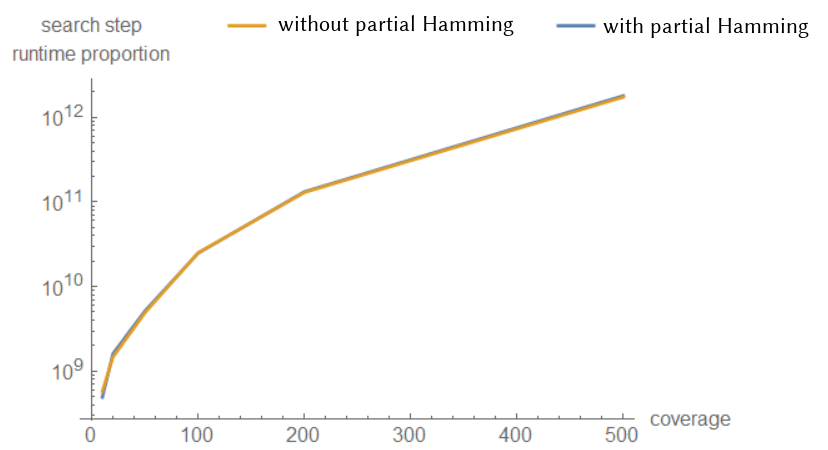
\includegraphics[width=.8\textwidth]{images/partial_hamming.png}
\caption{Comparative runtimes for executions with and without the `partial Hamming' modification across various values of coverage.}
\label{fig:partial_hamming}
\end{figure}

\subsection{Algorithm Extension Comparative Runtimes}
\label{extension_runtimes}

The \aspop{} implementation was built with the extensions from Section \ref{extensions} incorporated, enabled through the use of optional flags from the user. These extensions enrich the \gls{solution} set with new kinds of overlaps. The combination of several flags also yields unique solutions that cannot be found any other way. Of the three extensions (\gls{edit distance}, \glspl{reversal} and \glspl{inclusion}), use of reversals is most commonly advantageous for genome assembly. As such, it was used for tests throughout this work, but this need not be the case for the user.

Edit distance and inclusions are also not on by default; Although they are desirable in some cases, they are often not strictly necessary for sequence assembly, often avoided in part because they have a significant impact on runtime. Genome \gls{coverage} is shown to be a primary influence on runtime. As such, Figure \ref{fig:extensions} (a) shows the response of runtime to the use of the optional extensions, for otherwise the same problem instance; Although this figure seems to suggest that the enabling of edit distance simply scales up runtime by a constant factor, Figure \ref{fig:extensions} (b) shows that this is not the case. Using \textit{edit distance} fundamentally alters the ratios of work between the \gls{search step} and \gls{verification step} per run. Figure \ref{fig:cov} in Section \ref{phase2} would have us expect that (for edit distance disabled), the proportion of total runtime in Figure \ref{fig:extensions} (b) would fall below 50\% beyond the circa 500x \gls{coverage} mark. Unfortunately, with edit distance enabled, the runtime of this solver scales up considerably (as can be seen from (a)), forcing us to limit the coverage for this experiment to a maximum of 200x. We cannot extrapolate whether the edit-distance-enabled executions would experience runtimes with this same ratio of work in \gls{filter algorithm} steps as those of executions with edit distance disabled; Judging from the difference in behavior only within the 10x to 200x range, we would expect that the edit distance runs would likely not exhibit the `overtaking' behavior at 500x coverage seen in Figure \ref{fig:cov}.

\begin{figure}[!htb]
\centering
\makebox[\linewidth][c]{%
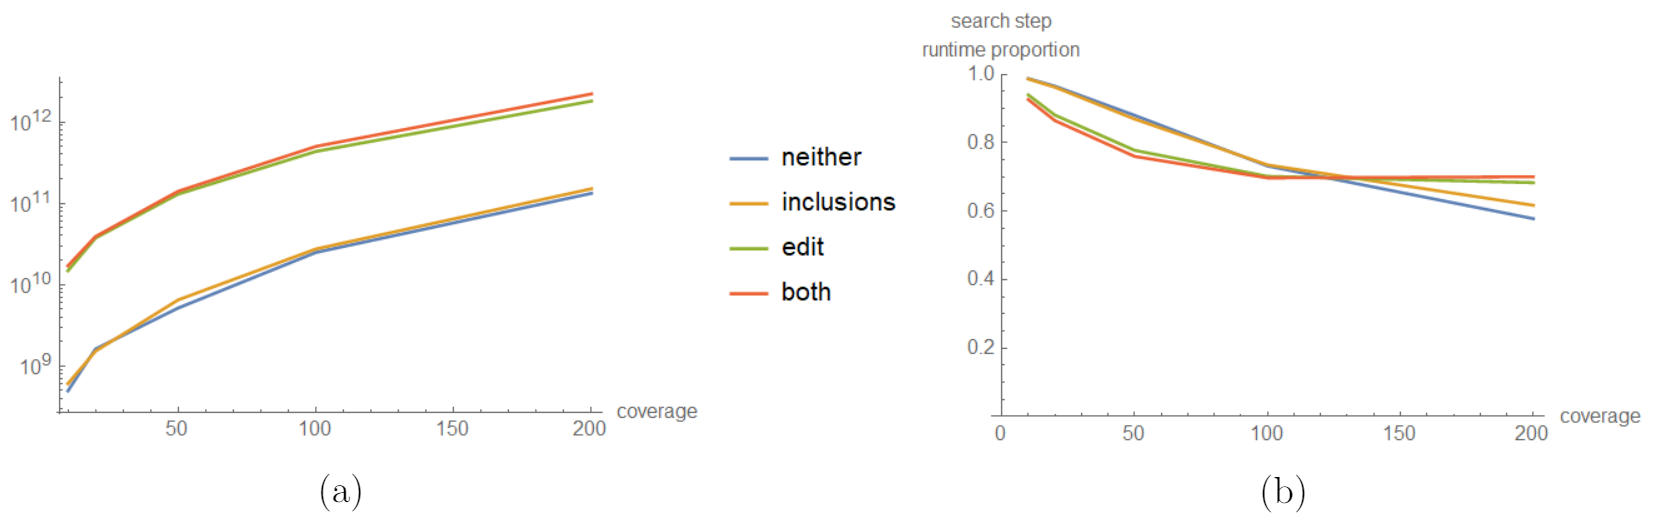
\includegraphics[width=1.15\textwidth]{images/extensions.png}
}
\caption[Runtime and runtime proportion of runs in response to coverage, with all combinations of optional flags enabling \textit{inclusions} and \textit{edit distance}.]{Runs in response to coverage, with all combinations of optional flags enabling \textit{inclusions} and \textit{edit distance} measured in terms of (a) Total runtime (b) Search step proportion of total runtime.}
\label{fig:extensions}
\end{figure}


\subsection{Runtime using \vali{}'s and Kucherov's Schemes}

Kucherov's \gls{suffix filter} algorithm introduced a new $S$ parameter (Explained in Section \ref{schemes:kuch}). In a nutshell, the choice of $S$ determines the number of \textit{redundant blocks} in the \gls{filter} associated with each search \gls{query} during the \gls{search step}. The trade-offs evident from choosing some $S$ over another yield an optimization problem, the nature of which is not immediately intuitive. 

Figure \ref{fig:schemes} demonstrates the runtime of executions using a modest viral-mix data set under the same parameters given by phase~1 in Section \ref{phase1}, in response to changing data set \gls{coverage}. \vali{}'s second algorithm resulted in significantly worse performance than Kucherov's with $S\leq{}2$ in all cases. This is consistent with Kucherov's own findings, as the \glspl{filter} in his scheme are more effective under these circumstances Additionally, Kucherov's algorithm makes use of a consistently-superior \gls{partitioning scheme}. The Kucherov run with $S=1$ behaves as the other Kucherov runs for extremely small data sets, but soon experiences \textit{extreme} slowdown in the higher-coverage run shown in Figure \ref{fig:schemes500}, much worse than that of the run using \vali{}'s second algorithm. This is a direct result of the \textit{short last block} problem explained in Section \ref{schemes:vali1} - \ref{schemes:kuch}. With $S=1$, no redundant blocks are given to the filters, resulting in the regrettable generation of hordes of \textit{spurious} \glspl{candidate}, as there are 0 completed blocks required by the \gls{candidate condition} in the \gls{query} search tree. This is especially evident in the shorter filters due to low $S$ values un-balancing the workload between filters. For this shorter run, \vali{}'s second algorithm still suffers  from its simple \gls{partitioning scheme}, relying on the work of more filters than would be necessary using Kucherov's partitioning scheme.

From all experiments conducted in this work, we observed a consistently superior runtime from Kucherov's algorithm with $S=2$. For this reason, $S=2$ is the value used elsewhere in the experiments. From Kucherov's own work, however, this trend might not continue to other problem instances with different properties beyond the bounds of our experiments \cite{kuch2014}.

\begin{figure}[!htb]
\centering
\makebox[\linewidth][c]{%
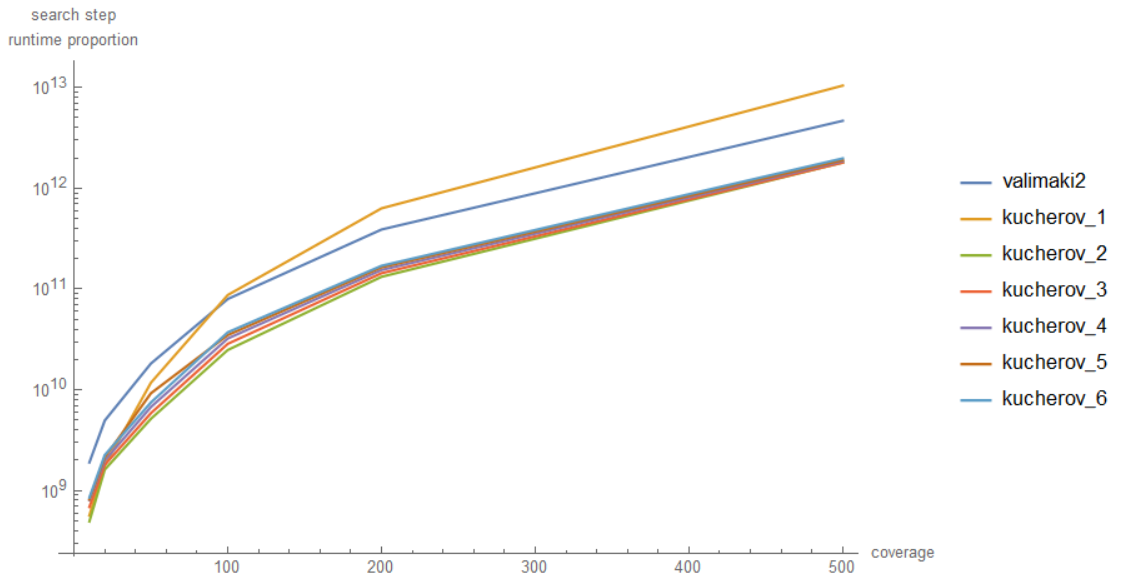
\includegraphics[width=1.0\textwidth]{images/schemes.png}
}
\caption{Comparative runtimes between \vali{}'s schemes, and Kucherov's schemes (using various values for parameter $S$), plotted in response to datasets with various values of coverage.}
\label{fig:schemes}
\end{figure}



\begin{figure}[!htb]
\centering
\makebox[\linewidth][c]{%
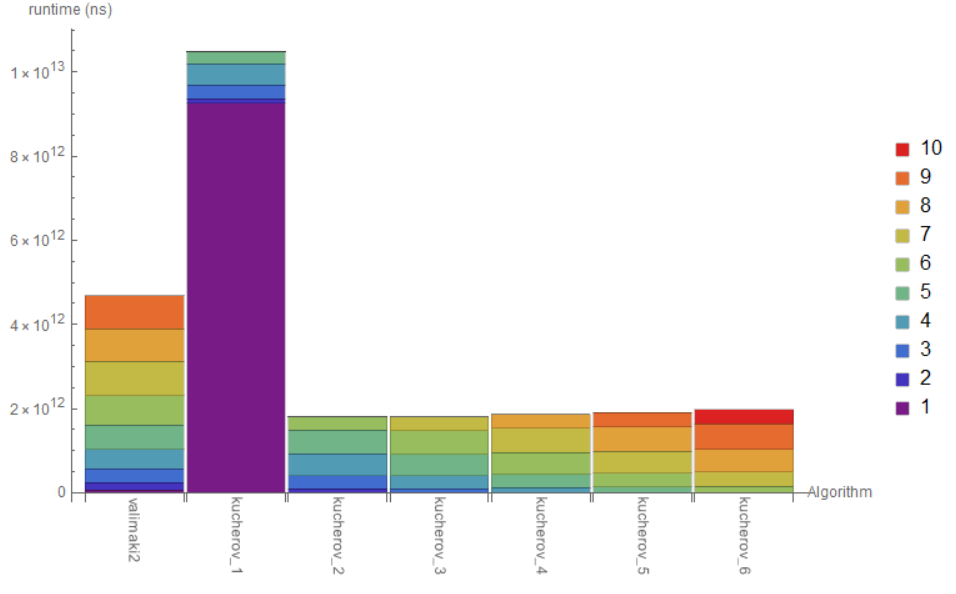
\includegraphics[width=0.9\textwidth]{images/schemes500.png}
}
\caption{Runtimes of filtering schemes of \vali{} and Kucherov, partitioned according to time per filter length, based on run `dataset\_coverage\_500x'.}
\label{fig:schemes500}
\end{figure}

\begin{figure}[!htb]
\centering
\makebox[\linewidth][c]{%
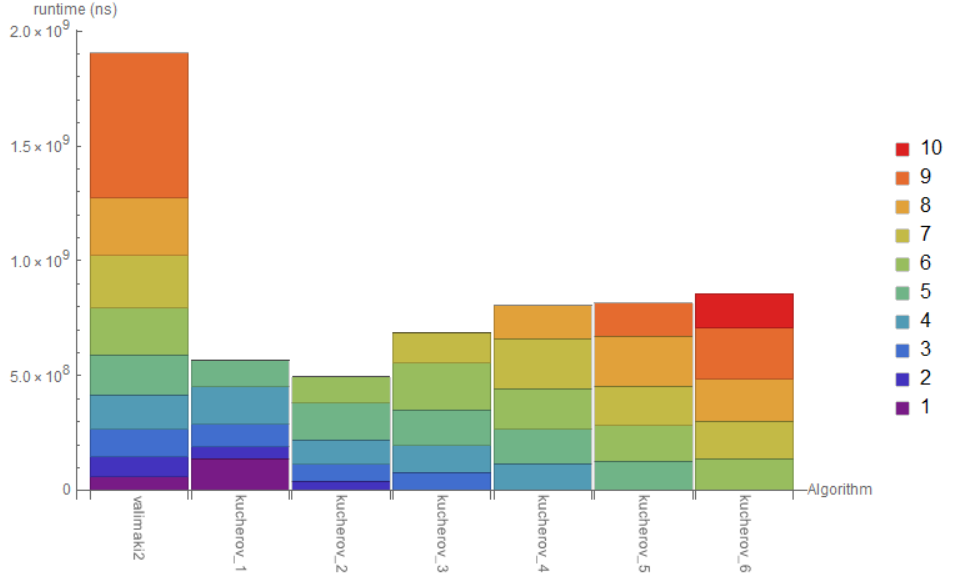
\includegraphics[width=0.9\textwidth]{images/schemes10.png}
}
\caption{Runtimes of filtering schemes of \vali{} and Kucherov, partitioned according to time per filter length, based on run `dataset\_coverage\_10x'.}
\label{fig:schemes10}
\end{figure}


\FloatBarrier
\subsection{Runtime on Full MHC Region of the Human Genome}
\label{fullmhc}

A final test of our program's speed tested its ability to handle larger data sets than were used for the numerous smaller tests. The the MHC region is located on chromosome 6, positions 28,477,797 - 33,448,354 (4,970,557 base pairs).

The run was under the same conditions as in phase 3 of the experiments, on a 24-core computer given 10 threads. After just under 25 hours, the program terminated with 1,051,648 solutions.

Unfortunately, the larger data sets showcased the differences in complexity classes between the solver. Compared to the second test in the phase 3 experiment, this data set came from a \gls{source genome} sequence 125x larger, and the run took 89,874 seconds up from 78. The run therefore took 1184x longer. By comparison, \textsc{blast} took 27 minutes to finish the same job, putting our \aspop{} solver to shame. Meanwhile, Minimap took just 34 seconds, now utterly blowing the competition out of the water in terms of speed.


\subsection{Prevalence of Pruned Nodes in Query Searches}
\label{aux:nodes}

This experiment intended to understand the practical difference between the worst-case and the typical case of the size of the \gls{query} search tree from the \gls{search step} of the \gls{suffix filter} algorithm. This section is somewhat meant as a \textit{foil} to the theoretical time complexity upper-bound defined in Section \ref{time_complexity}.

The implementation was temporarily modified to suppress pruning of \gls{query} search nodes that correspond with empty \gls{match location} sets. Instead, such nodes and all of their children are marked as `pruned' but otherwise retained. Counts of such nodes were printed to file, and the proportion computed for all searches in an execution in aggregate. It was immediately apparent during testing that the act of disabling pruning makes the solver significantly slower than before. Even the most trivial of data sets (40 \glspl{read} of 250bp) that usually takes less than a second to run didn't finish its execution in reasonable time. Thus, this experiment was run on a toy data set of generated reads with symbols sampled from a uniform distribution.

Table \ref{tab:nodes} shows the total prunable nodes in proportion to total nodes, using various combinations over ranges of \gls{read} length and number of input reads. No nodes are pruned for the 60-80 read length runs, as the search does not progress further than the first \gls{block} (with \bfit{t} set to 50). In runs with read length of 100 and beyond, an overwhelming proportion of the search tree is pruned. Naturally, the more massive search trees for longer read lengths produce more nodes; However, it becomes abundantly clear that as the search tree gets deeper, so too does the proportion of prunable nodes become even more overwhelming. In our experiment, the use of 5 significant figures was not sufficient to prevent this proportion from being indistinguishable from `1' for the largest read lengths. Although the number of reads indeed decreased the proportion of nodes pruned as expected (due to simply more \gls{text index} query hits), the proportion was modest, even between data sets with a 9-fold difference in number of reads.

As expected, the worst-case time complexity (which assumes only text index hits) is extremely pessimistic, and a user can expect a realistic execution to be \textit{lightening fast} by comparison.

\begin{table}
\centering
\caption[Proportion of nodes in query search trees pruned using Kucherov algorithm]{Proportion of nodes in query search trees pruned using Kucherov's algorithm on random data sets with $\bfit{e}=1.2\%$,  $S=2$, $\bfit{t}=50$ and reversals enabled. Read lengths (columns) ranged from 60 to 180; Number of input reads ranged from 10 to 90 (rows).\strut}
\begin{tabular}{|l||lllllll|}

\hline
 & 60 & 80 & 100 & 120 & 140 & 160 & 180 \\
\hline
\hline
10 & 0.0000 & 0.0000 & 0.9871 & 0.9909 & 0.9931 & 0.9945 & 1.0000 \\
30 & 0.0000 & 0.0000 & 0.9869 & 0.9908 & 0.9931 & 0.9945 & 1.0000 \\
90 & 0.0000 & 0.0000 & 0.9869 & 0.9908 & 0.9931 & 0.9945 & 1.0000 \\
\hline

\end{tabular}
\label{tab:nodes}
\end{table}